	\subsubsection{Regressions}
	Probably the most basic approach is simply running a regression with all the features as the independent variables and the a numeric representation of the classes as the dependent variable. Such an approach is shown in Equation \ref{regression}. Some threshold value between the classes must be determined since the estimate for the explained variable, will have a non-deterministic value. Regressions are primarily to be used as a benchmark for the other algorithms to measure up against.
	
	\begin{equation}
		\mathbb{E}(\hat{y} \ \vert \ \textbf{x}) \approx 
		\begin{cases}
			label = \text{News}, &\hat{y} \geq y^* \\
			label = \text{Not News},\ \ &\hat{y} < y^*
		\end{cases}
		\label{regression}
	\end{equation}
	
	\par
	\paragraph{Linear Regression}
		This method builds a linear dependency system between the explained variable (in this case, a numerical representation of the Class) and the explaining variables (Features). With the \textit{Bag-of-Words} approach, each parameter \textit{x} is a dummy variable indicating whether a given word \textit{m} is present in Tweet \textit{i}. The estimations parameters, which are denoted with $\beta_j$ are derived using Ordinary Least Squares. In itself, the linear regression estimation is a weak predictor for the purpose of classification, but it allows for calculating other useful statistics such as the coefficient of determination, commonly known as $R^2$. This static demonstrates the part of the variance that is explained using the provided variables and is also called 'goodness of fit'. We therefore strive to maximize it as much as possible. The more variance covered by our variables, the better we are able to predict the outcome of the classification. 
		
		\begin{figure}[h]
			\centering
			%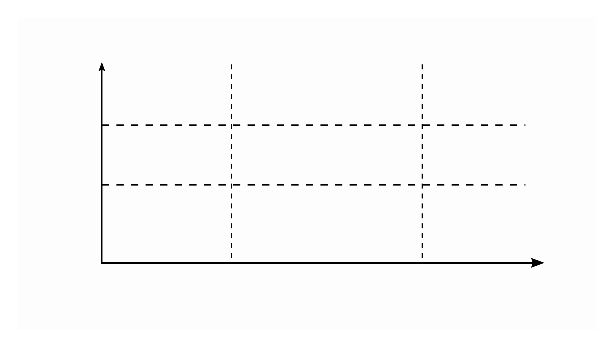
\includegraphics[width=0.8\textwidth]{methods}
			\scalebox{0.8}{\input{images/red_dist.eps_tex}}
			\captionsetup{width=0.8\textwidth}
			\caption{Distribution of predicted $ \hat{y} $ around the labels}
			\label{fig:y_dist_reg}
		\end{figure}
		
		Another point of interest is the distribution of predicted classifications $\hat{y}$. In an ideal scenario, the distribution of $\hat{y}$ would be concentrated around the numerical representations of the classes as in Figure \ref{fig:y_dist_reg}. The basic premise for the use of linear regressions as classification tools, where $ n $ is the number of observations, $ m $ is the number of features as presented in Equation \ref{lin_reg}.
	
	\begin{equation}
		y_i = \beta_1 x_{1i}+ \beta_2 x_{2i} + ... + \beta_m x_{mi} + \epsilon_i \ \ \ \ \ \ \ \ 
		\forall \ i \in [1,n].
		\label{lin_reg}
	\end{equation}
	
	\paragraph{Logistic Regression} Despite its name, the actual regression model executed here is linear, and is used primarily for classification rather than regression analysis (\cite{bishop2006logistic}). This regression scheme differs from linear firstly, in the fact, that the possible outcomes of the dependent variable are discreet rather than continuous. Secondly, the probabilities which describe the different outcomes of a regression instance, are modeled using a logistic function. The discrete outcomes can in turn be converted to labels, which in allows for a more fluent application as a classification tool and is therefore commonly employed in  Machine Learning. Logistic regression analysis is formally represented as follows in Equation \ref{logit}. The $x$ vector represents all explanatory variables, in our case, the Tweet features. The term error $\epsilon$ follows the standard logistic distribution, which also gives the regression its name. 
	
	\begin{equation}
		y = 
		\begin{cases}
		1 \ \  \beta_0 + \beta_1 x + \epsilon > 0 \\
		0 \ \  \text{else } 
		\end{cases} \text{         } \forall \  x = 
		\begin{pmatrix}x_1\\x_2\\...\\x_n \end{pmatrix}
		\label{logit}
	\end{equation}